\section*{Hadoop Blast}
 
By this point you should have gone over the sections concerning Hadoop Setup
and a few Hadoop programs. Now you are going to blend these applications by
implementing a parallel version of BLAST (Basic Local Alignment Search Tool:

\URL{http://blast.ncbi.nlm.nih.gov/Blast.cgi} 

using the programming
interfaces of the Hadoop MapReduce framework. Note that this application is
written in "Map-Only" fashion, which means no reduce code is necessary.

\subsection*{Deliverables} 

You are required to turn in the following items in a zip file
(username\_HadoopBlast.zip)

\begin{itemize} 
\item The source code of Hadoop Blast you implemented.
\item	Technical report (username\_HadoopBlast\_report.docx) that answers the
  following questions.

\begin{itemize}
\item What is Hadoop Distributed Cache and how is it used in this program? 
\item Write the two lines that put and get values from Distributed cache. Also
  include the method and class information.

\item In previous exercises we used Hadoop's TextInputFormat to feed in the file
  splits line by line to map tasks. In this program, however, we want to feed
    in a whole file to a single map task. What is the technique used to achieve
    this? Also, briefly explain what are the key and value pairs you receive as
    input to a map task and what methods are responsible for producing these
    pairs?

\item Do you think this particular implementation will work if the input files
  are larger than the default HDFS block size? Briefly explain why. [Hint: you
    can test what will happen by concatenating the same input file multiple
    times to create a larger input file in the resources/blast\_input folder]

\item	If you wanted to extend this program such that all output files will be
  concatenated into a single file, what key and value pairs would you need to
    emit from the map task? Also, how would you use these in the reduce that
    you would need to add?

\end{itemize}
\item	The 4 output FASTA files: celllines\_1.fa to celllines\_4.fa.
\end{itemize}


\subsection*{Evaluation} 

The point total for this exercise is 3, where the distribution is as follows:
\begin{itemize} 
\item	Completeness of your code and output (1 points)
\item	Correctness of written report (2 points)
\end{itemize}

\subsection*{Introduction}   

Hadoop-Blast is an advanced Hadoop program which helps BLAST, a bioinformatics
application, to utilize the computing capability of Hadoop. This exercise shows
the details of its implementation, and provides an example of how to handle
similar approaches in other applications.

BLAST is one of the most widely used bioinformatics applications written in
C++. The version we are using is v2.2.23, which houses new features and better
performance. The database used in the following settings is a subset of a full
8.5GB (nr) database; its full name is Non-redundant protein sequence database.
Optionally, for more details on how to run the BLAST binary, please see Big
Data for Science tutorial page for Blast Installation [NOT required for the
assignment].

In this exercise, we have provided a sketch code which contains just one java
class for you to implement:

\begin{itemize}
\item RunnerMap.java: The pleasingly-parallel/map-only Map class which takes
the prepackaged Blast (v2.2.23) Binary Program and optimized database from
Hadoop's Distributed Cache, then executes BLAST binary as java external process
with the assigned FASTA file. These are passed as key-value pairs of
\textbf{(filename, filepath on HDFS)} handled by a provided customized Hadoop
MapReduce InputFormat DataFileInputFormat.java.  
\end{itemize}

The detail dataflow can be seen in Figure~\ref{fig:blastdataflow}. You will
implement the RunnerMap.java, which copies the distributed cache and assigned
FASTA file to local, then run the BLAST binary with correct parameters.

\begin{figure}[!htbp]
\centering
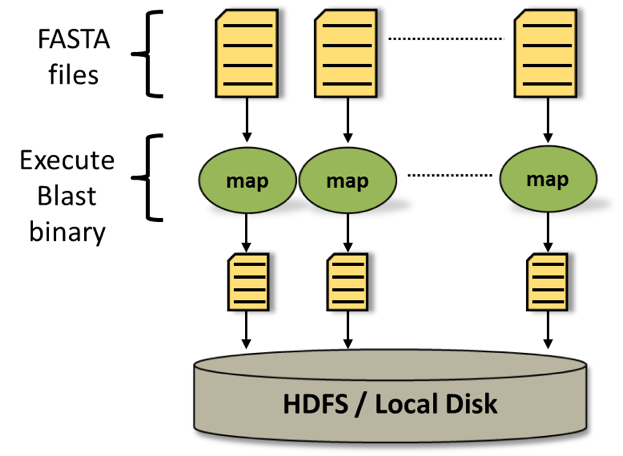
\includegraphics[width=8cm]{section/icloud/assignment/problems/exercise3/blastdataflow}
\caption{Hadoop Blast dataflow}
\label{fig:blastdataflow}
\end{figure}

Normally, for any Hadoop MapReduce program, input data is uploaded and stored
in the Hadoop Distributed File System (HDFS) before computation in order to
generate \textbf{(key, value)} pairs to the mapper. Initially, the BLAST input
data is a set of FASTA files located in the local file system. Then it will be
uploaded to the HDFS and distributed across the compute nodes. Hadoop framework
reads the application records from HDFS with the InputFormat interface and
generates \textbf{(key, value)} pair input streams; here, we use a provided
customized Hadoop MapReduce InputFormat DataFileInputFormat.java to generate
key-value pairs of \textbf{(filename, filepath on HDFS)}. For this Hadoop Blast
program, the map function initially sets up the distributed cache and generates
the two absolute location filepaths for Blast binary and Blast Database.
Afterwards it copies the assigned FASTA file to local disk by looking up the
file from HDFS and generating an absolute filepath. Once this is accomplished
and file dependencies are stored in the local disk, we call an external java
process and execute the Blast binary with the correct parameters. Finally, the
output FASTA file of Blast binary will be uploaded back to HDFS.

\subsection*{Sketch for Hadoop Blast}
You need to complete one file in the provided pacakge inside
"cgl/hadoop/apps/runner": RunnerMap.java. Code snapshots are shown below.

\lstinputlisting[language=Java]{section/icloud/assignment/problems/exercise3/RunnerMap.java}

In addition, if you need to understand the dataflow and main program, please
look into the DataAnalysis.java.

\lstinputlisting[language=Java]{section/icloud/assignment/problems/exercise3/DataAnalysis.java}


\subsection*{Edit}
The sketch code is stored within the provided VirtualBox image. Use linux text
editor vi/vim to add your code.

\begin{lstlisting}[language=bash]
$ cd /root/MoocHomeworks/HadoopBlast/
$ vim src/cgl/hadoop/apps/runner/RunnerMap.java
\end{lstlisting}

\subsection*{Compile and run your code}
Use the same one-click script compileAndExecHadoopBlast.sh as in prior
homework. Standard error messages such as compile errors, execution errors,
etc. will be redirected on the screen. Follow the same debugging format.

\begin{lstlisting}[language=bash]
$ cd /root/MoocHomeworks/HadoopBlast/
$ ./compileAndExecHadoopBlast.sh 
\end{lstlisting}

\subsection*{View the result} 
The result is generated at
/root/MoocHomeworks/HadoopBlast/output/HDFS\_blast\_output . There should be 4
output FASTA files with .fa extension

\begin{lstlisting}[language=bash]
$ cd /root/MoocHomeworks/HadoopBlast/output/HDFS_blast_output
$ ls
\end{lstlisting}
